\chapter{内积空间}
\label{chap:inner-product-spaces}

在$[-1,1]$上用常数近似$x^2$，最好的常数是多少？若用平方积分衡量误差，答案是$x^2$的平均值$\tfrac13$，误差函数$x^2-\tfrac13$与所有常数“垂直”。再问用$1,x,x^2,\ldots$的组合近似一个阶跃函数，项数越多误差是否越小、能否趋于零？这类问题需要的不只是误差的大小，还需要两个函数之间的角度。上一章的范数只提供前者，本章加入内积，研究正交带来的最佳逼近与无限展开。

本章先建立结构，再研究几何。第~\ref{sec:ipspace-inner-products}节把卷二的内积推广到函数与数列，固定实、复两种情形的约定，并说明内积怎样诱导范数、哪些范数不来自内积。第~\ref{sec:ipspace-hilbert-spaces}节把完备的内积空间称为Hilbert空间，第~\ref{sec:ipspace-l2-space}节以$L^2$与$\ell^2$说明内积、范数与完备性怎样同时成立。

后三节研究正交几何。第~\ref{sec:ipspace-orthogonal-projection}节证明Hilbert空间中闭子空间上的最佳逼近存在且唯一，它就是正交投影；这里完备性和闭性各有分工。第~\ref{sec:ipspace-orthonormal-bases}节定义完备正交系，说明它与代数基的区别，以及可分空间为什么有可数的正交基。第~\ref{sec:ipspace-orthogonal-expansions}节用正交系的系数写出展开，证明Bessel不等式与Parseval等式，并给出截断误差。

本章只研究内积带来的几何结构。连续线性泛函怎样表示为内积、正交投影作为算子的性质，分别在第~\ref{chap:linear-functionals}章和第~\ref{chap:linear-operators}章研究；三角函数系与小波的完备性在第~\ref{chap:fourier-transform}章和第~\ref{chap:wavelet-transform}章研究；正交展开的截断误差与函数光滑性的关系由第~\ref{chap:function-approximation}章处理；点值读取连续的Hilbert函数空间是第~\ref{chap:rkhs}章的对象。

\section{内积}
\label{sec:ipspace-inner-products}

\BookChapterRef{chap:inner-product-spaces}{卷二第4章“内积空间”}用内积定义了有限维空间中的长度、夹角和正交。内积的公理只涉及加法、数乘和取值，没有提到维数，所以可以原样放到函数和数列上。需要重新确认的是：函数上的内积具体长什么样，它给出的长度为什么是范数，以及哪些范数根本不可能来自内积。

\paragraph{内积的公理}
实空间中的内积是对称、双线性、正定的。复空间不能照搬这三条。若内积对两个变量都线性，把$x$换成$\mathrm ix$就得到
\[
 \langle\mathrm ix,\mathrm ix\rangle=\mathrm i^2\langle x,x\rangle=-\langle x,x\rangle,
\]
于是$\langle x,x\rangle$与$\langle\mathrm ix,\mathrm ix\rangle$不可能都是正数。所以复内积改用共轭对称，并且只对一个变量线性。本书与卷二一致，约定对第二个变量线性、对第一个变量共轭线性。

\begin{definition}[内积与内积空间]
\label{def:ipspace-inner-product}
设$V$是$\mathbb K$上的线性空间。映射$\langle\cdot,\cdot\rangle:V\times V\to\mathbb K$称为$V$上的\term{内积}（inner product），若对所有$f,g,h\in V$与$a,b\in\mathbb K$，
\begin{align}
 \langle h,af+bg\rangle&=a\langle h,f\rangle+b\langle h,g\rangle,
 \label{eq:ipspace-axiom-linear}\\
 \langle g,f\rangle&=\overline{\langle f,g\rangle},
 \label{eq:ipspace-axiom-conjugate}\\
 \langle f,f\rangle&\geq0,
 \label{eq:ipspace-axiom-positive}
\end{align}
且$\langle f,f\rangle=0$当且仅当$f=0$。这三条分别称为对第二个变量线性、共轭对称和正定性。配备内积的线性空间称为\term{内积空间}（inner-product space）。
\end{definition}

前两条合起来给出对第一个变量的共轭线性：
\[
 \langle af+bg,h\rangle=\bar a\langle f,h\rangle+\bar b\langle g,h\rangle.
\]
共轭对称还说明$\langle f,f\rangle$等于自己的共轭，总是实数，所以第三条的“$\geq0$”有意义。实空间中共轭不起作用，三条公理就是卷二的对称、双线性和正定性。

\paragraph{函数与数列上的内积}
先看点积怎样变成积分。把$[-1,1]$等分成$N$小段，步长$h=2/N$，取各段中点$x_1,\ldots,x_N$。函数$f$在这些点上读出一个$N$维向量$(f(x_1),\ldots,f(x_N))$，这正是“函数是无限维向量”的有限截取。两个这样的向量作点积，再乘以步长，得到
\begin{equation}
 h\sum_{i=1}^N\overline{f(x_i)}\,g(x_i)\ \xrightarrow{\ N\to\infty\ }\ \int_{-1}^1\overline{f(x)}\,g(x)\,dx .
 \label{eq:ipspace-riemann-dot}
\end{equation}
乘以$h$是必要的：不乘的话，分量越多点积越大，没有极限。

下面用$f(x)=1+x$、$g(x)=x$和$N=4$算一遍。此时$h=\tfrac12$，四个中点是$\pm\tfrac14,\pm\tfrac34$，两个函数读出的向量是
\[
 f\mapsto(0.25,\,0.75,\,1.25,\,1.75),\qquad g\mapsto(-0.75,\,-0.25,\,0.25,\,0.75).
\]
逐分量相乘再相加，得到点积
\[
 -0.1875-0.1875+0.3125+1.3125=1.25 .
\]
乘以步长$h=\tfrac12$，得到$0.625$。

精确的积分是
\[
 \int_{-1}^1(1+x)x\,dx=\int_{-1}^1x\,dx+\int_{-1}^1x^2\,dx=\frac23 .
\]
取$N=8$和$N=16$，同样的计算分别给出$0.65625$和$0.6640625$，逐渐接近$\tfrac23$。图~\ref{fig:ipspace-sampled-dot-product}画出了$N=4$时的情形：左边是两组读出的分量，右边每个矩形的高是一对分量的乘积，矩形的带符号总面积就是式~\eqref{eq:ipspace-riemann-dot}左边的和。

\begin{BookInlineFigure}
  \centering
  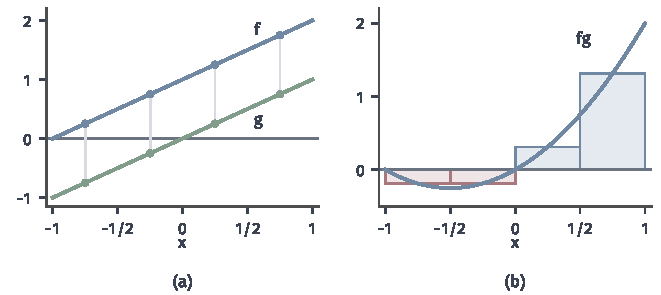
\includegraphics[width=112mm]{figures/04-spaces-measures-and-geometry/03-function-spaces/matplotlib/ipspace-sampled-dot-product/figure.pdf}
  \caption{从点积到积分内积，$f=1+x$（蓝），$g=x$（绿），$N=4$。(a)四个中点上读出的分量。(b)矩形的高是分量的乘积$f(x_i)g(x_i)$（负值用红色），宽是步长$\tfrac12$，带符号总面积$0.625$；曲线是$fg$，其下带符号面积是内积$\tfrac23$。}
  \label{fig:ipspace-sampled-dot-product}
\end{BookInlineFigure}

这个极限提示了$C[a,b]$上的内积：
\begin{equation}
 \langle f,g\rangle=\int_a^b\overline{f(x)}\,g(x)\,dx .
 \label{eq:ipspace-continuous-inner-product}
\end{equation}
实函数时共轭可以省去。对第二个变量的线性和共轭对称来自积分的线性。

正定性要用到连续性。被积函数非负，所以
\[
 \langle f,f\rangle=\int_a^b\lvert f\rvert^2\,dx\geq0 .
\]
若$f(x_0)\neq0$，由连续性存在长度为正的小区间，在其上$\lvert f\rvert\geq\tfrac12\lvert f(x_0)\rvert$，积分至少是区间长度乘$\tfrac14\lvert f(x_0)\rvert^2$，严格为正。

这里类比也开始失效。有限维向量的每个分量都带着正的权重，改动一个分量，长度就变了。积分内积中单个点的权重趋于零，改动一个点的值不影响积分。在连续函数上，连续性阻止了这种改动；一旦离开连续函数，正定性就要靠第~\ref{sec:ipspace-l2-space}节的等价类来恢复。

数列是更直接的无限维向量，下标集是$\mathbb N_+$，内积就是点积把求和号延伸到无穷：$\sum_k\overline{x_k}y_k$。麻烦在于和可能发散，比如$(1,1,1,\ldots)$与自己的点积。在有限支撑数列空间$c_{00}$上不会有这个问题，求和只有有限项非零，
\begin{equation}
 \langle x,y\rangle=\sum_k\overline{x_k}\,y_k
 \label{eq:ipspace-c00-inner-product}
\end{equation}
是内积。容纳无穷多项非零的数列要等到第~\ref{sec:ipspace-l2-space}节的$\ell^2$。

共轭在函数上同样不能省略。在$[-\pi,\pi]$上取$f(x)=e^{\mathrm ix}$，这是一个处处模长为$1$的非零函数。若不取共轭，
\[
 \int_{-\pi}^{\pi}f(x)\,f(x)\,dx=\int_{-\pi}^{\pi}e^{2\mathrm ix}\,dx=0,
\]
一个非零函数与自己的“内积”竟然为零。取共轭后被积函数变成$\lvert e^{\mathrm ix}\rvert^2=1$，于是$\langle f,f\rangle=2\pi$。

若$\langle f,g\rangle=0$，称$f$与$g$\term{正交}（orthogonal）。这里的“垂直”指乘积的整体积分为零，与两条曲线在平面上的交角无关。在$[-1,1]$上，$1$与$x$正交，$1$与$x^2$不正交，因为
\[
 \int_{-1}^1x\,dx=0,\qquad \int_{-1}^1x^2\,dx=\frac23 .
\]
正交还依赖积分区间：换到$[0,1]$上，$\int_0^1x\,dx=\tfrac12$，$1$与$x$就不再正交了。

\paragraph{Cauchy--Schwarz不等式与诱导范数}
内积给出长度$\lVert f\rVert=\sqrt{\langle f,f\rangle}$。要说明它是范数，关键在三角不等式，而三角不等式依赖下面这个不等式。

它的几何图景是：$\mathbb R^3$中把$f$投影到$g$所在的直线上，垂线段的长度不小于零，由此得到$\cos\theta$的绝对值不超过$1$。证明就是把这幅图写成计算，用到的只有内积公理，与维数无关。

\begin{theorem}[Cauchy--Schwarz不等式]
\label{thm:ipspace-cauchy-schwarz}
在内积空间中，对所有$f,g$，
\begin{equation}
 \lvert\langle f,g\rangle\rvert\leq\lVert f\rVert\,\lVert g\rVert ,
 \label{eq:ipspace-cauchy-schwarz}
\end{equation}
等号当且仅当$f,g$线性相关。
\end{theorem}

\begin{proof}
若$g=0$，两边都为零，$f,g$线性相关。下面设$g\neq0$。

取$f$在$g$方向上的影子$\alpha g$，其中$\alpha=\langle g,f\rangle/\lVert g\rVert^2$。这个系数使余量$f-\alpha g$与$g$正交：
\[
 \langle g,f-\alpha g\rangle=\langle g,f\rangle-\alpha\lVert g\rVert^2=0 .
\]

展开余量长度的平方时，先把第二个变量拆开。含$g$的那一项因为上面的正交关系而消失，于是
\[
 \lVert f-\alpha g\rVert^2=\langle f-\alpha g,f\rangle=\lVert f\rVert^2-\bar\alpha\langle g,f\rangle .
\]

代入$\bar\alpha=\langle f,g\rangle/\lVert g\rVert^2$。$\langle f,g\rangle$与$\langle g,f\rangle$互为共轭，乘积是模的平方，于是
\[
 0\leq\lVert f-\alpha g\rVert^2=\lVert f\rVert^2-\frac{\lvert\langle f,g\rangle\rvert^2}{\lVert g\rVert^2}.
\]
移项开方即得不等式。等号成立当且仅当$\lVert f-\alpha g\rVert=0$，即$f=\alpha g$；反过来，若$f=cg$，直接代入可知$\alpha=c$，等号成立。
\end{proof}

用$[0,1]$上的$f=1$、$g=x$核对一下。三个内积是
\[
 \langle f,g\rangle=\frac12,\qquad \lVert f\rVert^2=1,\qquad \lVert g\rVert^2=\frac13 .
\]
不等式成为$\tfrac12\leq\tfrac1{\sqrt3}\approx0.577$。影子的系数是$\alpha=\tfrac12\big/\tfrac13=\tfrac32$，余量$1-\tfrac32x$的长度平方是
\[
 \int_0^1\Bigl(1-\frac32x\Bigr)^2dx=1-\frac32+\frac34=\frac14,
\]
与证明中的公式给出的$1-\tfrac34$相同。

在实空间中，式~\eqref{eq:ipspace-cauchy-schwarz}保证下面的比值落在$[-1,1]$内，可以用它定义函数之间的夹角：
\[
 \cos\theta=\frac{\langle f,g\rangle}{\lVert f\rVert\,\lVert g\rVert}.
\]
上面的$1$与$x$在$[0,1]$上的夹角满足$\cos\theta=\tfrac{\sqrt3}2$，即$\theta=30^\circ$；在$[-1,1]$上内积为零，夹角是$90^\circ$。

三角不等式现在可以推出。把$\lVert f+g\rVert^2$按内积展开，再用Cauchy--Schwarz不等式放大交叉项：
\[
 \begin{aligned}
 \lVert f+g\rVert^2&=\lVert f\rVert^2+2\operatorname{Re}\langle f,g\rangle+\lVert g\rVert^2\\
 &\leq\lVert f\rVert^2+2\lVert f\rVert\,\lVert g\rVert+\lVert g\rVert^2\\
 &=(\lVert f\rVert+\lVert g\rVert)^2 .
 \end{aligned}
\]
齐次性$\lVert cf\rVert=\lvert c\rvert\,\lVert f\rVert$与正定性直接来自内积公理。所以每个内积空间都是赋范空间，这个范数称为内积的\term{诱导范数}（induced norm）。在$C[a,b]$上，它就是平方积分大小$\bigl(\int_a^b\lvert f\rvert^2\,dx\bigr)^{1/2}$。

Cauchy--Schwarz不等式还说明内积对两个变量连续。把差拆成只改一个变量的两项：
\[
 \langle f_n,g_n\rangle-\langle f,g\rangle=\langle f_n-f,g_n\rangle+\langle f,g_n-g\rangle .
\]
对每一项用不等式~\eqref{eq:ipspace-cauchy-schwarz}，得到
\begin{equation}
 \lvert\langle f_n,g_n\rangle-\langle f,g\rangle\rvert\leq\lVert f_n-f\rVert\,\lVert g_n\rVert+\lVert f\rVert\,\lVert g_n-g\rVert .
 \label{eq:ipspace-inner-continuity}
\end{equation}
若$f_n\to f$、$g_n\to g$，$\lVert g_n\rVert$有界，右边趋于零，所以$\langle f_n,g_n\rangle\to\langle f,g\rangle$。后面凡是在极限中保持正交关系，用的都是这一点。

\paragraph{平行四边形恒等式}
内积范数比一般范数多一条性质。在平面上，平行四边形两条对角线的平方和等于四条边的平方和。这条几何事实在内积空间中照样成立：
\begin{equation}
 \lVert f+g\rVert^2+\lVert f-g\rVert^2=2\lVert f\rVert^2+2\lVert g\rVert^2 ,
 \label{eq:ipspace-parallelogram}
\end{equation}
称为\term{平行四边形恒等式}（parallelogram identity）。验证时把左边两项按内积展开，交叉项$2\operatorname{Re}\langle f,g\rangle$与$-2\operatorname{Re}\langle f,g\rangle$相互抵消，剩下的正是右边。

一般的范数未必满足它，因此未必来自内积。在$C[0,1]$上取一致范数，令$f=1$、$g=x$。这时$f+g=1+x$的最大值是$2$，$f-g=1-x$的最大值是$1$，于是
\[
 \lVert f+g\rVert_\infty^2+\lVert f-g\rVert_\infty^2=4+1=5 .
\]
而$\lVert f\rVert_\infty=\lVert g\rVert_\infty=1$，右边是
\[
 2\lVert f\rVert_\infty^2+2\lVert g\rVert_\infty^2=4 .
\]

$L^1$范数同样不满足。在$L^1[0,1]$中取两半区间的指示函数$f=\mathbf 1_{[0,1/2]}$、$g=\mathbf 1_{(1/2,1]}$，有
\[
 \lVert f+g\rVert_1=\lVert f-g\rVert_1=1,\qquad \lVert f\rVert_1=\lVert g\rVert_1=\frac12 .
\]
左边等于$2$，右边等于$1$。两个范数都违反式~\eqref{eq:ipspace-parallelogram}，所以没有任何内积能诱导它们。

反过来，满足平行四边形恒等式的范数一定来自内积。实情形下这个内积只能是
\begin{equation}
 \langle f,g\rangle=\frac14\bigl(\lVert f+g\rVert^2-\lVert f-g\rVert^2\bigr) ,
 \label{eq:ipspace-polarization}
\end{equation}
因为按内积展开右边，正好只剩$\langle f,g\rangle$。证明这个式子确实定义了内积，需要由恒等式逐步推出可加性，再把齐次性从有理数推广到实数，篇幅较长，读者可在泛函分析教材中查阅Jordan--von Neumann定理。本章只用正方向：内积范数满足式~\eqref{eq:ipspace-parallelogram}，它将是第~\ref{sec:ipspace-orthogonal-projection}节证明最近点存在的关键。

\section{Hilbert空间}
\label{sec:ipspace-hilbert-spaces}

内积空间是赋范空间，因而可以谈柯西列与完备性。下一节之后的最佳逼近与无限展开都要从柯西列得到极限，所以需要把完备性与内积放在一起。

\begin{definition}[Hilbert空间]
\label{def:ipspace-hilbert}
若内积空间在诱导范数下完备，即诱导度量满足第~\ref{chap:metric-spaces}章的完备性，称它为\term{Hilbert空间}（Hilbert space）。
\end{definition}

按定义，Hilbert空间就是范数来自内积的Banach空间。反过来不成立：上一节说明一致范数与$L^1$范数不满足平行四边形恒等式，而第~\ref{chap:normed-spaces}章证明了$C[0,1]$在一致范数下完备、$L^1[0,1]$完备，所以它们是Banach空间，却不是Hilbert空间。“有没有内积”和“是否完备”是两个独立的判断。

有限维内积空间总是完备的，因为有限维赋范空间在任意范数下都完备。所以有限维时，内积空间与Hilbert空间是同一回事，卷二的全部正交理论都在完备空间中进行。无限维时，完备性要对每个具体空间单独证明；下面两个例子说明它确实可能不成立。

\paragraph{有限支撑数列}
在$c_{00}$上取内积$\langle x,y\rangle=\sum_k\overline{x_k}y_k$。令
\begin{equation*}
x^{(N)}=(1,\tfrac12,\ldots,\tfrac1N,0,0,\ldots)\in c_{00}.
\end{equation*}
对$M>N$，
\[
 \lVert x^{(M)}-x^{(N)}\rVert^2=\sum_{k=N+1}^M\frac1{k^2}\leq\sum_{k>N}\frac1{k^2}\to0,
\]
所以$(x^{(N)})$是柯西列。

它在$c_{00}$中没有极限。若$\lVert x^{(N)}-y\rVert\to0$对某个$y\in c_{00}$成立，由于每个坐标的差都不超过范数，$\lvert x^{(N)}_k-y_k\rvert\leq\lVert x^{(N)}-y\rVert$，每个坐标都收敛，所以$y_k=\lim_Nx^{(N)}_k=1/k$对所有$k$成立。这样的$y$有无穷多项非零，不在$c_{00}$中，矛盾。所以$c_{00}$是不完备的内积空间。

\paragraph{连续函数与平方积分}
在$C[-1,1]$上取实内积$\langle f,g\rangle=\int_{-1}^1fg\,dx$，诱导范数记为$\lVert\cdot\rVert_2$。连续斜坡
\[
 g_n(x)=\begin{cases}-1,&x\leq-1/n,\\ nx,&\lvert x\rvert<1/n,\\ 1,&x\geq1/n\end{cases}
\]
越来越陡，越来越像符号函数$\operatorname{sgn}$，如图~\ref{fig:ipspace-ramp-step}所示。对$m>n$，两函数只在$\lvert x\rvert<1/n$上不同且差的绝对值不超过$1$，所以$\lVert g_n-g_m\rVert_2^2\leq2/n$，$(g_n)$是柯西列。

\begin{figure}[!htb]
  \centering
  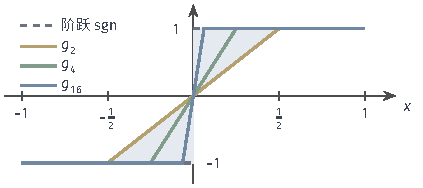
\includegraphics[width=71.6mm]{figures/02-abstract-mathematics/03-function-spaces/tikz/c1-ramp-step/figure.pdf}
  \caption{连续斜坡$g_n$逼近符号函数$\operatorname{sgn}$。$g_n$在$\lvert x\rvert\geq1/n$处与$\operatorname{sgn}$相同，只在宽为$2/n$的区间内线性过渡；阴影是$n=2$时二者之差所在的区域。直接积分得$\int_{-1}^1(g_n-\operatorname{sgn})^2\,dx=\tfrac{2}{3n}\to0$，但$\operatorname{sgn}$在$0$处跳跃，没有连续代表。}
  \label{fig:ipspace-ramp-step}
\end{figure}

它在$C[-1,1]$中没有$\lVert\cdot\rVert_2$极限。若连续函数$g$满足$\lVert g_n-g\rVert_2\to0$，任取$\delta\in(0,1)$，当$n>1/\delta$时$g_n$在$[\delta,1]$上恒为$1$，于是$\int_\delta^1(1-g)^2\,dx\leq\lVert g_n-g\rVert_2^2\to0$，由连续性$g=1$在$[\delta,1]$上成立；同理$g=-1$在$[-1,-\delta]$上成立。$\delta$任意，$g$在$0$处不可能连续，矛盾。这与第~\ref{chap:normed-spaces}章积分范数下的不完备例子是同一机制，只是误差改用平方累计。

两个例子中，柯西列的“极限”都存在，只是不在原来的集合里：前者是平方可和的数列$(1/k)$，后者是平方可积的阶跃函数。下一节的$\ell^2$与$L^2$正是把这些极限都收进来的空间。

\section{\texorpdfstring{$L^2$}{L2}空间}
\label{sec:ipspace-l2-space}

上一节的两个不完备例子分别缺少平方可和的数列和平方可积的阶跃函数。第~\ref{chap:function-normed-spaces}章已经在几乎处处等价类上建立了$L^2$，并证明它在$L^2$范数下完备。接下来只需在$L^2$上定义内积，并核对它诱导的正是这个范数。本节固定测度空间$(X,\mathcal A,\mu)$。

\paragraph{\texorpdfstring{$L^2$}{L2}内积}
点积推广到函数时写成乘积的积分，首先要保证这个积分有意义。有限维的和总是有限的，无限维时要靠条件。对$f,g\in L^2(\mu)$，Hölder不等式在$p=q=2$时给出
\[
 \int_X\lvert\bar fg\rvert\,d\mu=\int_X\lvert f\rvert\,\lvert g\rvert\,d\mu\leq\lVert f\rVert_2\,\lVert g\rVert_2<\infty,
\]
所以$\bar fg$可积。

于是可以令
\begin{equation}
 \langle f,g\rangle=\int_X\bar fg\,d\mu ,
 \label{eq:ipspace-l2-inner-product}
\end{equation}
实函数时共轭可以省去。复值函数的积分按第~\ref{chap:integration}章的规定，实部、虚部分别积分。

这个定义不依赖代表的选择。若$f'\sim_\mu f$、$g'\sim_\mu g$，则$\bar f'g'$与$\bar fg$只在零测集$\{f'\neq f\}\cup\{g'\neq g\}$上可能不同，积分相同。所以$\langle\cdot,\cdot\rangle$是等价类上定义合理的映射。

\paragraph{内积公理与诱导范数}
对第二个变量的线性来自积分的线性，共轭对称来自$\overline{\int\bar fg\,d\mu}=\int f\bar g\,d\mu$。正定性值得细看：被积函数非负，所以
\[
 \langle f,f\rangle=\int_X\lvert f\rvert^2\,d\mu\geq0 ,
\]
且它为零当且仅当$\lvert f\rvert^2=0$几乎处处，也就是$[f]$是零元素。

正是等价类使正定性成立。若在普通函数上计算，只在一点非零的函数也会使$\langle f,f\rangle=0$，正定性就失败了。第~\ref{sec:ipspace-inner-products}节说过，积分内积中单个点没有权重；把函数换成等价类，就是承认这件事，不再区分只差一个零测集的函数。

诱导范数是
\[
 \sqrt{\langle f,f\rangle}=\Bigl(\int_X\lvert f\rvert^2\,d\mu\Bigr)^{1/2}=\lVert f\rVert_2 ,
\]
恰好是第~\ref{chap:function-normed-spaces}章的$L^2$范数。那里已经证明$L^2(\mu)$在这个范数下完备，所以下面的定理不需要新的论证。

\begin{theorem}[$L^2$是Hilbert空间]
\label{thm:ipspace-l2-hilbert}
对任意测度空间，$L^2(\mu)$配以式~\eqref{eq:ipspace-l2-inner-product}的内积是Hilbert空间。
\end{theorem}

上一节的阶跃例子在这里有了去处。$\operatorname{sgn}$的等价类属于$L^2[-1,1]$。$g_n$与$\operatorname{sgn}$只在$\lvert x\rvert<1/n$上不同，左右两半对称，所以
\[
 \lVert g_n-\operatorname{sgn}\rVert_2^2=2\int_0^{1/n}(1-nx)^2\,dx=\frac{2}{3n}\to0 .
\]
斜坡列在$L^2[-1,1]$中收敛到$\operatorname{sgn}$。

\paragraph{\texorpdfstring{$\ell^2$}{l2}空间}
取$X=\mathbb N_+$与计数测度，积分变成求和，等价类就是数列本身，得到
\begin{equation}
 \begin{gathered}
 \ell^2=\Bigl\{x=(x_k):\ \sum_{k\geq1}\lvert x_k\rvert^2<\infty\Bigr\},\\
 \langle x,y\rangle=\sum_{k\geq1}\overline{x_k}\,y_k .
 \end{gathered}
 \label{eq:ipspace-ell2}
\end{equation}
这是最字面意义上的“无限维向量空间”：元素就是$[a_1,a_2,\ldots]$，内积就是点积，唯一的新要求是长度有限。级数的绝对收敛来自计数测度下的Hölder不等式。由定理~\ref{thm:ipspace-l2-hilbert}，$\ell^2$是Hilbert空间。

$c_{00}$是$\ell^2$的子空间，内积是限制后的内积，上一节的柯西列$x^{(N)}$在$\ell^2$中收敛到$(1/k)$。$c_{00}$的不完备，只是因为它没有包含这些极限。有限维的$\mathbb K^d$可以看作只有前$d$项非零的数列，这时$\ell^2$内积就是卷二的标准内积。

$\ell^2$与$L^2[-1,1]$的差别值得留意。两者都是Hilbert空间，但$\ell^2$的下标是离散的，每个坐标都带着权重$1$，读取第$k$个坐标是连续的操作；$L^2[-1,1]$中单点没有权重，读取函数在某一点的值根本没有定义。

\paragraph{\texorpdfstring{$L^2$}{L2}中的正交}
函数的正交是乘积的积分为零。图~\ref{fig:ipspace-integral-orthogonality}在$L^2[-1,1]$中对照了两种情形：$1\cdot x$在正负半区间上的带符号面积相互抵消；$1\cdot x^2$处处非负，面积无处抵消。同样的对称性说明，$[-1,1]$上任何偶函数都与任何奇函数正交，因为乘积是奇函数，积分为零。

\begin{BookInlineFigure}
  \centering
  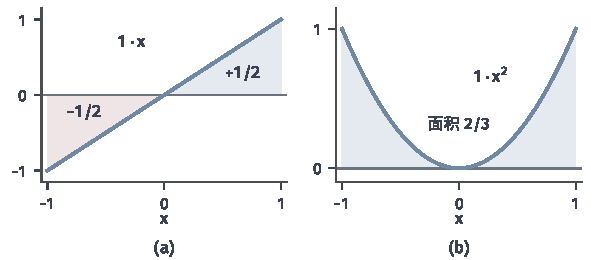
\includegraphics[width=100mm]{figures/04-spaces-measures-and-geometry/03-function-spaces/matplotlib/ipspace-integral-orthogonality/figure.pdf}
  \caption{积分内积下的正交。$[-1,1]$上取Lebesgue测度，曲线是两个函数的乘积，阴影是带符号面积。(a)$1\cdot x$的正负面积各为$\tfrac12$，内积为$0$，$1$与$x$正交。(b)$1\cdot x^2$处处非负，内积为$\tfrac23$，$1$与$x^2$不正交。}
  \label{fig:ipspace-integral-orthogonality}
\end{BookInlineFigure}

复情形的典型例子是复指数。在$L^2[-\pi,\pi]$中，对整数$j,k$，第一个变量取共轭，指数相减：
\[
 \begin{aligned}
 \langle e^{\mathrm ijx},e^{\mathrm ikx}\rangle
 &=\int_{-\pi}^{\pi}e^{-\mathrm ijx}e^{\mathrm ikx}\,dx\\
 &=\int_{-\pi}^{\pi}e^{\mathrm i(k-j)x}\,dx .
 \end{aligned}
\]
当$j=k$时被积函数为$1$，积分为$2\pi$。当$j\neq k$时，$e^{\mathrm imx}$（$m=k-j\neq0$）在一个周期上积分为零，因为它的原函数$e^{\mathrm imx}/(\mathrm im)$在两端取值相同。

所以$\{e^{\mathrm ikx}/\sqrt{2\pi}\}_{k\in\mathbb Z}$两两正交且长度为$1$。这一族是否足以表示$L^2[-\pi,\pi]$的每个元素，是第~\ref{chap:fourier-transform}章的问题。

\section{正交投影}
\label{sec:ipspace-orthogonal-projection}

章首问：在$L^2[-1,1]$中用常数近似$x^2$，哪个常数最好？更一般地，给定Hilbert空间$H$中的一个子空间$M$与一个目标$f$，能否在$M$中找到离$f$最近的元素。有限维中，卷二证明了最近点存在、唯一，并且误差与子空间正交。无限维中新的问题是：逼近距离的下确界能否被取到。本节证明，只要$H$完备、$M$闭，答案就是肯定的。

\paragraph{正交补}
先给出“与整个子空间垂直”的元素组成的集合。对子集$M\subseteq H$，令
\[
 M^\perp=\{g\in H:\ \langle m,g\rangle=0\ \text{对所有}\ m\in M\},
\]
称为$M$的\term{正交补}（orthogonal complement）。它是线性子空间，因为内积对第二个变量线性。它还是闭集：若$g_n\in M^\perp$且$g_n\to g$，由内积的连续性，$\langle m,g\rangle=\lim_n\langle m,g_n\rangle=0$对每个$m\in M$成立。所以无论$M$本身是否闭，$M^\perp$总是闭线性子空间。

\paragraph{最佳逼近的存在与唯一}
设$M\subseteq H$是线性子空间，$f\in H$，记
\[
 d=d(f,M)=\inf_{m\in M}\lVert f-m\rVert .
\]
下确界总是存在的。问题在于是否有$m\in M$恰好取到它：在无限维中，越来越好的近似可能没有极限，极限也可能离开$M$。下面的定理说明，完备性和闭性分别排除这两种情况，而平行四边形恒等式保证越来越好的近似确实彼此接近。

\begin{theorem}[闭子空间上的最佳逼近]
\label{thm:ipspace-best-approximation}
设$H$是Hilbert空间，$M\subseteq H$是闭线性子空间。则对每个$f\in H$，存在唯一的$m_*\in M$使$\lVert f-m_*\rVert=d(f,M)$。
\end{theorem}

\begin{proof}
取$m_n\in M$使$\lVert f-m_n\rVert^2<d^2+1/n$，称为极小化序列。

第一步，极小化序列是柯西列。对$f-m_j$与$f-m_k$用平行四边形恒等式~\eqref{eq:ipspace-parallelogram}，
\[
 \lVert m_j-m_k\rVert^2=2\lVert f-m_j\rVert^2+2\lVert f-m_k\rVert^2-4\Bigl\lVert f-\frac{m_j+m_k}2\Bigr\rVert^2 .
\]
$M$是线性子空间，中点$\tfrac{m_j+m_k}2$在$M$中，所以最后一项中的范数平方至少为$d^2$。于是$\lVert m_j-m_k\rVert^2<2(d^2+\tfrac1j)+2(d^2+\tfrac1k)-4d^2=\tfrac2j+\tfrac2k$，$(m_n)$是柯西列。

第二步，极限存在且留在$M$中。$H$完备，所以$m_n$收敛到某个$m_*\in H$；$M$闭，所以$m_*\in M$。由范数的连续性，$\lVert f-m_*\rVert=\lim_n\lVert f-m_n\rVert=d$。

第三步，唯一性。若$m_*,m_*'\in M$都取到$d$，则二者交替排列成的序列$m_*,m_*',m_*,m_*',\ldots$也是极小化序列，由第一步是柯西列，所以$m_*=m_*'$。
\end{proof}

三个条件各有分工。平行四边形恒等式说明：若两个点离$f$都几乎是最近的，它们彼此必然很近，这一步依赖内积，一般Banach空间中最近点可能不唯一，也可能不存在。$H$的完备性给出极小化序列的极限，$M$的闭性保证这个极限没有离开$M$。实际上前两步只用到$M$自身的完备性：若$M$在限制后的范数下完备，即使$H$不完备，结论也成立，这适用于任意内积空间中的有限维子空间。

\paragraph{误差正交与正交投影}
最近点还可以用正交关系刻画，这是计算它的实用方法。

\begin{theorem}[正交刻画]
\label{thm:ipspace-orthogonality-characterization}
设$H$是Hilbert空间，$M\subseteq H$是闭线性子空间，$f\in H$，$m_*\in M$。则$\lVert f-m_*\rVert=d(f,M)$当且仅当$f-m_*\in M^\perp$。此时对任意$m\in M$，
\begin{equation}
 \lVert f-m\rVert^2=\lVert f-m_*\rVert^2+\lVert m_*-m\rVert^2 .
 \label{eq:ipspace-pythagoras}
\end{equation}
\end{theorem}

\begin{proof}
设$m_*$取到$d$，记$r=f-m_*$。任取$m\in M$与$t\in\mathbb K$，$m_*+tm\in M$，所以$\lVert r\rVert^2\leq\lVert r-tm\rVert^2=\lVert r\rVert^2-2\operatorname{Re}\bigl(t\langle r,m\rangle\bigr)+\lvert t\rvert^2\lVert m\rVert^2$。取$t=s\,\overline{\langle r,m\rangle}$，$s>0$为实数，得$2s\lvert\langle r,m\rangle\rvert^2\leq s^2\lvert\langle r,m\rangle\rvert^2\lVert m\rVert^2$。两边除以$s$再令$s\to0$，得$\langle r,m\rangle=0$。所以$r\in M^\perp$。

反过来，设$r=f-m_*\in M^\perp$。对任意$m\in M$，$m_*-m\in M$与$r$正交，展开$\lVert r+(m_*-m)\rVert^2$时交叉项为零，得式~\eqref{eq:ipspace-pythagoras}。于是$\lVert f-m\rVert\geq\lVert f-m_*\rVert$，等号当且仅当$m=m_*$，$m_*$是最近点。
\end{proof}

式~\eqref{eq:ipspace-pythagoras}是勾股关系：$f$、$m_*$、$m$三点构成以$m_*$为直角顶点的直角三角形，见图~\ref{fig:ipspace-projection-geometry}。它不仅说明$m_*$最近，还定量地给出任何其他候选多出的误差，恰为它到$m_*$的距离平方。

\begin{figure}[!htb]
  \centering
  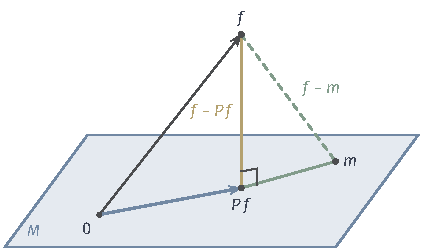
\includegraphics[width=71.7mm]{figures/02-abstract-mathematics/03-function-spaces/tikz/c1-projection-geometry/figure.pdf}
  \caption{闭子空间上的正交投影（示意）。平面代表闭子空间$M$，$Pf$是$M$中离$f$最近的点，误差$f-Pf$与$M$垂直。对$M$中任意另一点$m$，三点构成直角三角形，$\lVert f-m\rVert^2=\lVert f-Pf\rVert^2+\lVert Pf-m\rVert^2$，所以$m$离$f$更远。}
  \label{fig:ipspace-projection-geometry}
\end{figure}

\begin{definition}[正交投影]
\label{def:ipspace-orthogonal-projection}
设$M$是Hilbert空间$H$的闭线性子空间。把定理~\ref{thm:ipspace-best-approximation}中的最近点$m_*$记为$P_Mf$，称为$f$在$M$上的\term{正交投影}（orthogonal projection）。
\end{definition}

\paragraph{正交分解}
由定理~\ref{thm:ipspace-orthogonality-characterization}，每个$f\in H$都可以写成
\[
 f=P_Mf+(f-P_Mf),\qquad P_Mf\in M,\quad f-P_Mf\in M^\perp .
\]
这种分解是唯一的：若$f=m+g=m'+g'$，$m,m'\in M$，$g,g'\in M^\perp$，则$m-m'=g'-g$同时属于$M$与$M^\perp$，与自己正交，只能为零。所以$H$中每个元素唯一地分成$M$中的部分与$M^\perp$中的部分，记作$H=M\oplus M^\perp$。

由勾股关系还得到$\lVert f\rVert^2=\lVert P_Mf\rVert^2+\lVert f-P_Mf\rVert^2$，所以$\lVert P_Mf\rVert\leq\lVert f\rVert$。$P_M$的线性也可以从正交刻画读出：$af+bg-(aP_Mf+bP_Mg)$是两个$M^\perp$中元素的组合，仍在$M^\perp$中，所以$aP_Mf+bP_Mg$就是$af+bg$的投影。把$P_M$作为线性算子研究，是第~\ref{chap:linear-operators}章的内容。

\paragraph{向常数投影}
回到章首的问题。在$L^2[-1,1]$中取$M=\operatorname{span}\{1\}$，它是一维子空间，因而闭。由正交刻画，$c$是最佳常数当且仅当$\langle1,f-c\rangle=\int_{-1}^1(f-c)\,dx=0$，即
\[
 c=\frac12\int_{-1}^1f(x)\,dx ,
\]
最佳常数就是平均值。对$f=x^2$，$P_Mf=\tfrac13$，误差$x^2-\tfrac13$与$1$正交，距离平方为
\[
 \int_{-1}^1\Bigl(x^2-\frac13\Bigr)^2dx=\frac25-\frac49+\frac29=\frac8{45}.
\]
由式~\eqref{eq:ipspace-pythagoras}，任何其他常数$c$的误差平方都是$\tfrac8{45}+2(c-\tfrac13)^2$。

\paragraph{闭性不能去掉}
定理~\ref{thm:ipspace-best-approximation}中的闭性是必要的。在$\ell^2$中取$M=c_{00}$，它是线性子空间但不闭。令$f=(1,\tfrac12,\tfrac13,\ldots)\in\ell^2$。截断$x^{(N)}\in c_{00}$满足$\lVert f-x^{(N)}\rVert^2=\sum_{k>N}1/k^2\to0$，所以$d(f,c_{00})=0$。若下确界被某个$m\in c_{00}$取到，则$\lVert f-m\rVert=0$，$f=m$有无穷多项非零，矛盾。最近点不存在：每个有限支撑数列都可以再改进，却没有最好的那一个。

\paragraph{与一般闭凸集的分工}
定理~\ref{thm:ipspace-best-approximation}的第一、二步只用到两件事：中点$\tfrac{m_j+m_k}2$仍在$M$中，以及$M$闭。所以把$M$换成任意非空闭凸集$C$，同样的论证给出最近点的存在与唯一。但定理~\ref{thm:ipspace-orthogonality-characterization}用到了$m_*+tm\in M$对所有$t$成立，这是线性子空间的性质；对闭凸集，正交条件要换成变分不等式$\operatorname{Re}\langle f-m_*,c-m_*\rangle\leq0$（$c\in C$），投影也不再是线性映射。闭凸集上的投影及其在优化算法中的使用，可参考\BookChapterRef{chap:nonsmooth-composite-optimization}{卷五第4章“非光滑与复合优化”}。本章只处理线性子空间。

\section{正交基}
\label{sec:ipspace-orthonormal-bases}

有限维内积空间中，标准正交基让坐标的计算变得简单：第$j$个坐标就是与第$j$个基向量的内积。无限维中，第~\ref{chap:functions-as-vectors}章已经看到代数基只允许有限组合，常常无法写出，也不适合谈论级数。本节换一种要求：不要求每个元素都是有限个方向的组合，只要求它能被这些方向的有限组合以任意精度逼近。

\paragraph{标准正交系}
先给出两两正交、长度为$1$的一族元素。

\begin{definition}[标准正交系]
\label{def:ipspace-orthonormal-system}
内积空间$H$中的一族元素$\{e_i\}_{i\in I}$称为\term{标准正交系}（orthonormal system），若对所有$i,j\in I$，
\[
 \langle e_i,e_j\rangle=\delta_{i,j}=\begin{cases}1,&i=j,\\0,&i\neq j.\end{cases}
\]
\end{definition}

标准正交系总是线性无关的：若$\sum_{k=1}^nc_ke_{i_k}=0$，与$e_{i_j}$作内积得$c_j=0$。$\ell^2$中的标准单位列$\{e_k\}_{k\geq1}$是标准正交系；上一节的$\{e^{\mathrm ikx}/\sqrt{2\pi}\}_{k\in\mathbb Z}$是$L^2[-\pi,\pi]$中的标准正交系。

\paragraph{Gram--Schmidt正交化}
标准正交系可以从任意线性无关的序列造出来。设$u_1,u_2,\ldots$线性无关，依次令
\[
 v_k=u_k-\sum_{j<k}\langle e_j,u_k\rangle e_j,\qquad e_k=\frac{v_k}{\lVert v_k\rVert}.
\]
$v_k$是$u_k$减去它在$e_1,\ldots,e_{k-1}$方向上的分量，与之前的方向都正交：对$i<k$，$\langle e_i,v_k\rangle=\langle e_i,u_k\rangle-\langle e_i,u_k\rangle=0$。$v_k\neq0$，因为否则$u_k$属于$\operatorname{span}\{e_1,\ldots,e_{k-1}\}=\operatorname{span}\{u_1,\ldots,u_{k-1}\}$，与线性无关矛盾。归纳可知$\operatorname{span}\{e_1,\ldots,e_k\}=\operatorname{span}\{u_1,\ldots,u_k\}$对每个$k$成立。这就是卷二的\term{Gram--Schmidt正交化}（Gram--Schmidt orthogonalization），每一步只涉及有限维子空间，所以可以无限地进行下去。

在$L^2[-1,1]$中对$1,x,x^2,x^3$执行这一过程。$\lVert1\rVert^2=2$，$e_0=1/\sqrt2$。$x$与$1$正交，$\lVert x\rVert^2=\tfrac23$，$e_1=\sqrt{3/2}\,x$。对$x^2$，$\langle e_0,x^2\rangle=\tfrac{\sqrt2}3$，$\langle e_1,x^2\rangle=0$，于是$v_2=x^2-\tfrac13$，这正是上一节向常数投影的误差，$\lVert v_2\rVert^2=\tfrac8{45}$，故
\[
 e_2=\sqrt{\tfrac{45}{8}}\Bigl(x^2-\frac13\Bigr)=\sqrt{\tfrac58}\,(3x^2-1).
\]
对$x^3$，它与偶函数$e_0,e_2$正交，$\langle e_1,x^3\rangle e_1=\tfrac32\cdot\tfrac25x=\tfrac35x$，于是$v_3=x^3-\tfrac35x$，$\lVert v_3\rVert^2=\tfrac27-\tfrac{12}{25}+\tfrac6{25}=\tfrac8{175}$，故$e_3=\sqrt{7/8}\,(5x^3-3x)$。

这些是归一化的\term{Legendre多项式}（Legendre polynomials）。图~\ref{fig:ipspace-legendre-gram-schmidt}对照了正交化前后的函数：单项式$x^2$与$1$、$x^3$与$x$在大部分区间上走向相近，远不正交；正交化后，每个$e_k$恰比前一个多一次变号。

\begin{figure}[!htb]
  \centering
  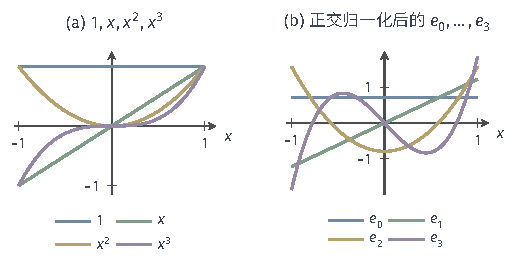
\includegraphics[width=87.3mm]{figures/02-abstract-mathematics/03-function-spaces/tikz/c1-legendre-gram-schmidt/figure.pdf}
  \caption{在$L^2[-1,1]$中对单项式做Gram--Schmidt正交化。(a)$1,x,x^2,x^3$，例如$\langle1,x^2\rangle=\tfrac23\neq0$；(b)得到的$e_0=1/\sqrt2$，$e_1=\sqrt{3/2}\,x$，$e_2=\sqrt{5/8}\,(3x^2-1)$，$e_3=\sqrt{7/8}\,(5x^3-3x)$，两两正交且范数为$1$，$e_k$在$(-1,1)$内恰有$k$个零点。}
  \label{fig:ipspace-legendre-gram-schmidt}
\end{figure}

\paragraph{完备正交系}
一个标准正交系“够不够用”，看它的有限组合能否逼近每个元素。$\{e_i\}$的有限线性组合全体记为$\operatorname{span}\{e_i\}$，它在$H$中的闭包记为$\overline{\operatorname{span}}\{e_i\}$，称为\term{闭线性张成}（closed linear span）。

\begin{definition}[完备正交系]
\label{def:ipspace-complete-orthonormal-system}
若Hilbert空间$H$中的标准正交系$\{e_i\}_{i\in I}$满足$\overline{\operatorname{span}}\{e_i\}=H$，称它为$H$的\term{完备正交系}（complete orthonormal system），也称\term{标准正交基}（orthonormal basis）或正交基。
\end{definition}

这里的“完备”与空间的完备是两个不同的概念：前者说正交系的方向够用，后者说柯西列有极限。“基”字也要小心理解。代数基要求每个元素恰是有限个基元素的组合；正交基只要求每个元素是有限组合的范数极限，允许通过极限逼近。下一节将说明，这样的极限可以写成按范数收敛的级数。

$\ell^2$中的标准单位列是完备正交系。对$x\in\ell^2$，截断$x^{(N)}=\sum_{k\leq N}x_ke_k\in\operatorname{span}\{e_k\}$满足
\[
 \lVert x-x^{(N)}\rVert^2=\sum_{k>N}\lvert x_k\rvert^2\to0,
\]
因为收敛级数的尾和趋于零。所以$\operatorname{span}\{e_k\}=c_{00}$在$\ell^2$中稠密。但$\{e_k\}$不是$\ell^2$的代数基：$(1,\tfrac12,\tfrac13,\ldots)\in\ell^2$有无穷多项非零，不是有限个$e_k$的组合。

\paragraph{完备性的正交判据}
判断一个标准正交系是否完备，常用的办法是看还有没有被它遗漏的方向。

\begin{theorem}[完备正交系的判据]
\label{thm:ipspace-completeness-criterion}
设$\{e_i\}_{i\in I}$是Hilbert空间$H$中的标准正交系。则它是完备正交系，当且仅当与每个$e_i$都正交的元素只有零。
\end{theorem}

\begin{proof}
记$M=\overline{\operatorname{span}}\{e_i\}$，它是闭线性子空间。设$M=H$，$g$与每个$e_i$正交。由内积的线性，$g$与$\operatorname{span}\{e_i\}$正交；由内积的连续性，$g$也与其闭包$M=H$正交，特别地$\langle g,g\rangle=0$，$g=0$。

反过来，设$M\neq H$，取$f\notin M$。由第~\ref{sec:ipspace-orthogonal-projection}节，$g=f-P_Mf$属于$M^\perp$，且$g\neq0$，因为$P_Mf\in M$而$f\notin M$。这个$g$与每个$e_i$正交，所以判据的条件不成立。
\end{proof}

判据的“必要”方向只用到内积的连续性，“充分”方向用到了正交投影，从而用到了完备性与闭性。例如在$L^2[-1,1]$中，偶次的归一化Legendre多项式$e_0,e_2,e_4,\ldots$组成一个无穷的标准正交系，但$x$是奇函数，与每个偶函数正交，而$x\neq0$。所以这个系不完备：方向有无穷多个，却遗漏了全部奇函数。

全体Legendre多项式$\{e_k\}_{k\geq0}$是否完备，取决于多项式能否在$L^2[-1,1]$中逼近每个元素。这需要两步逼近：连续函数在$L^2[-1,1]$中稠密，多项式又能一致逼近连续函数。这两步属于第~\ref{chap:function-approximation}章，这里不给出证明，只指出结论：Legendre多项式是$L^2[-1,1]$的完备正交系。

\paragraph{可分空间的可数正交基}
要用级数$\sum_jc_je_j$表示每个元素，正交基最好是可数的。第~\ref{chap:topological-spaces}章把具有可数稠密子集的空间称为\term{可分}（separable）空间。下面说明，对Hilbert空间而言，“有可数的正交基”与“可分”是一回事。

\begin{theorem}[可分Hilbert空间的正交基]
\label{thm:ipspace-separable-basis}
设$H$是可分Hilbert空间，$H\neq\{0\}$。则$H$有至多可数的标准正交基，并且$H$中每个标准正交系都至多可数。
\end{theorem}

\begin{proof}
取可数稠密子集$\{u_k\}_{k\geq1}$。依次检查各项，删去能由前面保留的项线性表示的项，得到一个线性无关的序列（有限或无限），其张成空间与$\operatorname{span}\{u_k\}$相同。对它做Gram--Schmidt正交化，得到标准正交系$\{e_j\}$，其张成空间仍与$\operatorname{span}\{u_k\}$相同。这个张成空间包含稠密集$\{u_k\}$，所以在$H$中稠密，$\{e_j\}$是至多可数的完备正交系。

再设$\{e_i\}_{i\in I}$是任意标准正交系。对$i\neq j$，$\lVert e_i-e_j\rVert^2=\lVert e_i\rVert^2+\lVert e_j\rVert^2=2$。所以以各$e_i$为中心、半径$\tfrac{\sqrt2}2$的开球两两不交。每个开球都含有稠密集$\{u_k\}$中的点，不同的球含有不同的点，于是$i\mapsto$（球中某个$u_k$的下标$k$）是$I$到$\mathbb N_+$的单射，$I$至多可数。
\end{proof}

反方向也成立：若$H$有可数的正交基$\{e_j\}$，则系数取有理数（复情形取实部、虚部为有理数）的有限组合构成可数集，并且在$H$中稠密，所以$H$可分。$\ell^2$有可数的正交基$\{e_k\}$，因而可分；由上面所述的Legendre多项式的完备性，$L^2[-1,1]$也可分。不可分的Hilbert空间也存在，那时正交基不可数，下一节的级数需要改写为不可数族的求和，本书不展开。

\section{正交展开}
\label{sec:ipspace-orthogonal-expansions}

有了可数的标准正交系，就可以写出级数$\sum_jc_je_j$。第~\ref{chap:functions-as-vectors}章指出，级数要回答三个问题：是否收敛、表示哪些元素、系数是否唯一。本节在Hilbert空间中用范数收敛回答它们：系数由内积给出，有限截断是正交投影，完备正交系给出收敛的展开与能量恒等式，不完备的正交系只恢复它张成的那一部分。

本节设$H$是Hilbert空间，$\{e_j\}$是有限或可数的标准正交系，下标按$j=1,2,\ldots$排列。对$f\in H$，称
\[
 c_j=\langle e_j,f\rangle
\]
为$f$关于$\{e_j\}$的系数。

\paragraph{有限截断是正交投影}
先看只保留有限个方向时的情形。记$M_n=\operatorname{span}\{e_1,\ldots,e_n\}$，它是有限维子空间，因而闭，第~\ref{sec:ipspace-orthogonal-projection}节的结论适用。

\begin{theorem}[有限截断]
\label{thm:ipspace-finite-truncation}
对$f\in H$与$n\geq1$，令$s_n=\sum_{j=1}^nc_je_j$。则$s_n=P_{M_n}f$，并且
\begin{equation}
 \lVert f-s_n\rVert^2=\lVert f\rVert^2-\sum_{j=1}^n\lvert c_j\rvert^2 .
 \label{eq:ipspace-truncation-error}
\end{equation}
\end{theorem}

\begin{proof}
$s_n\in M_n$。对每个$k\leq n$，由标准正交性$\langle e_k,s_n\rangle=\sum_jc_j\langle e_k,e_j\rangle=c_k$，所以$\langle e_k,f-s_n\rangle=c_k-c_k=0$。$f-s_n$与$M_n$的每个基元素正交，因而与$M_n$正交；由正交刻画，$s_n=P_{M_n}f$。再由勾股关系$\lVert f\rVert^2=\lVert s_n\rVert^2+\lVert f-s_n\rVert^2$与$\lVert s_n\rVert^2=\sum_{j\leq n}\lvert c_j\rvert^2$即得式~\eqref{eq:ipspace-truncation-error}。
\end{proof}

这个定理说明，用内积计算的系数就是$M_n$中的最佳选择：在$e_1,\ldots,e_n$的所有组合中，$s_n$离$f$最近。增加一个方向时，已经算好的系数不需要修改，误差平方恰好减少新系数的模平方。若$\{e_j\}$只是线性无关而不正交，这两件事都不成立，系数要重新解一个Gram矩阵方程组。

\paragraph{Bessel不等式}
式~\eqref{eq:ipspace-truncation-error}的左边非负，所以对每个$n$都有$\sum_{j\leq n}\lvert c_j\rvert^2\leq\lVert f\rVert^2$。令$n\to\infty$，得到下面的不等式。

\begin{theorem}[Bessel不等式]
\label{thm:ipspace-bessel}
对$f\in H$，$\sum_j\lvert\langle e_j,f\rangle\rvert^2\leq\lVert f\rVert^2$。
\end{theorem}

非负项级数的部分和有界，所以级数收敛，和不超过这个界。特别地$c_j\to0$：任何元素在越来越靠后的正交方向上的分量都越来越小。这一结论只用到正交系，不要求它完备，也不要求$H$完备。

\paragraph{级数的收敛与和}
Bessel不等式说明系数平方可和。反过来，平方可和的系数总能给出一个收敛的级数，它的和就是$f$在闭张成空间上的投影。

\begin{theorem}[正交展开]
\label{thm:ipspace-orthogonal-expansion}
设$M=\overline{\operatorname{span}}\{e_j\}$。
\begin{enumerate}
 \item 对数列$(a_j)$，级数$\sum_ja_je_j$依范数收敛，当且仅当$\sum_j\lvert a_j\rvert^2<\infty$；此时$\lVert\sum_ja_je_j\rVert^2=\sum_j\lvert a_j\rvert^2$。
 \item 对$f\in H$，级数$\sum_jc_je_j$依范数收敛，其和为$P_Mf$。
\end{enumerate}
\end{theorem}

\begin{proof}
（1）记部分和$t_n=\sum_{j\leq n}a_je_j$。对$n>m$，由标准正交性，$\lVert t_n-t_m\rVert^2=\sum_{m<j\leq n}\lvert a_j\rvert^2$。所以$(t_n)$是柯西列当且仅当$\sum_j\lvert a_j\rvert^2$的部分和是柯西数列，即级数收敛。$H$完备，柯西列收敛；反之收敛列是柯西列。范数等式由$\lVert t_n\rVert^2=\sum_{j\leq n}\lvert a_j\rvert^2$与范数的连续性得到。

（2）由Bessel不等式和（1），$s_n=\sum_{j\leq n}c_je_j$收敛到某个$s$。每个$s_n\in M$，$M$闭，所以$s\in M$。对固定的$k$与$n\geq k$，$\langle e_k,f-s_n\rangle=0$；令$n\to\infty$，由内积的连续性得$\langle e_k,f-s\rangle=0$。于是$f-s$与$\operatorname{span}\{e_j\}$正交，再由连续性与其闭包$M$正交。由正交刻画，$s=P_Mf$。
\end{proof}

（1）中的“仅当”方向不需要完备性，“当”方向需要：在不完备的$c_{00}$中，$\sum_ka_ke_k$对$a_k=1/k$就不收敛。（2）也回答了唯一性：若$\sum_ja_je_j=g$依范数收敛，与$e_k$作内积并取极限，得$a_k=\langle e_k,g\rangle$，系数只能是内积系数。由于（2）对$\{e_j\}$的任何排列都成立，和总是$P_Mf$，所以级数的和不依赖求和次序。

\paragraph{完备正交系：展开与Parseval等式}
若$\{e_j\}$是完备正交系，则$M=H$，$P_Mf=f$，得到最重要的情形。

\begin{theorem}[Parseval等式]
\label{thm:ipspace-parseval}
设$\{e_j\}$是$H$的完备正交系，$f,g\in H$，$c_j=\langle e_j,f\rangle$，$d_j=\langle e_j,g\rangle$。则
\[
 f=\sum_jc_je_j\quad(\text{依范数}),\qquad \lVert f\rVert^2=\sum_j\lvert c_j\rvert^2,\qquad \langle f,g\rangle=\sum_j\overline{c_j}\,d_j .
\]
\end{theorem}

\begin{proof}
展开式由定理~\ref{thm:ipspace-orthogonal-expansion}（2）与$M=H$得到。在式~\eqref{eq:ipspace-truncation-error}中令$n\to\infty$，左边趋于零，得范数等式，称为\term{Parseval等式}（Parseval identity）。对内积，$\langle s_n,t_n\rangle=\sum_{j\leq n}\overline{c_j}d_j$，其中$t_n$是$g$的部分和；由内积的连续性，左边趋于$\langle f,g\rangle$。
\end{proof}

Parseval等式说明，当正交基为可数无穷时，取系数$f\mapsto(c_j)$把$H$一一地映成$\ell^2$，并保持内积：每个$f$给出平方可和的系数，每个平方可和的系数列由定理~\ref{thm:ipspace-orthogonal-expansion}（1）给出唯一的元素。所以一个具有可数正交基的无限维Hilbert空间，在选定正交基后，与$\ell^2$只有记号的差别，就像有限维内积空间选定标准正交基后与$\mathbb K^d$只有记号的差别一样。

由式~\eqref{eq:ipspace-truncation-error}与Parseval等式，截断误差可以直接从系数读出：
\begin{equation}
 \lVert f-s_n\rVert^2=\sum_{j>n}\lvert c_j\rvert^2 ,
 \label{eq:ipspace-tail-error}
\end{equation}
即系数平方的尾和。误差随$n$单调下降并趋于零，下降的快慢完全由系数衰减的快慢决定。

\paragraph{不完备时只恢复闭张成中的部分}
若$\{e_j\}$不完备，展开的和是$P_Mf$而不是$f$，正交补$M^\perp$中的分量永远丢失。Bessel不等式与Parseval等式之间的差$\lVert f\rVert^2-\sum_j\lvert c_j\rvert^2=\lVert f-P_Mf\rVert^2$，正是丢失部分的能量。

回到偶次Legendre多项式。设$E$为$L^2[-1,1]$中几乎处处满足$f(-x)=f(x)$的元素组成的子空间。任意$f$都可以写成$f(x)=\tfrac{f(x)+f(-x)}2+\tfrac{f(x)-f(-x)}2$，前者是偶函数，属于$E$，后者是奇函数，与$E$正交。由正交分解的唯一性，$P_Ef(x)=\tfrac{f(x)+f(-x)}2$，并且$E$就是这个投影的像。偶次Legendre多项式是偶函数，它们的闭张成含于$E$。反过来，对$f\in E$，奇次的$e_k$是奇函数，$\langle e_k,f\rangle=0$；由上一节所述的全体Legendre多项式的完备性，$f$的展开只含偶次项，所以$f$属于偶次Legendre多项式的闭张成。于是这个闭张成恰为$E$，只用偶次方向展开时，和就是$P_Ef$。

取$f=e^x$，得$P_Ef=\cosh x$，丢失的部分是奇部$\sinh x$，见图~\ref{fig:ipspace-even-odd-projection}。距离平方为
\[
 \int_{-1}^1\sinh^2x\,dx=\frac{\sinh2}{2}-1\approx0.813 ,
\]
无论加入多少偶次方向都无法减小。

\begin{figure}[!htb]
  \centering
  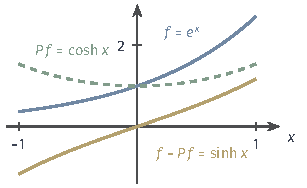
\includegraphics[width=51.9mm]{figures/02-abstract-mathematics/03-function-spaces/tikz/c1-even-odd-projection/figure.pdf}
  \caption{向偶函数子空间的正交投影。$[-1,1]$上$f(x)=e^x$，投影$P_Ef=\cosh x$为其偶部，误差$f-P_Ef=\sinh x$为奇函数，与每个偶函数正交。只用偶次方向展开$e^x$时，误差始终至少为$\lVert\sinh\rVert_2\approx0.90$。}
  \label{fig:ipspace-even-odd-projection}
\end{figure}

\paragraph{截断误差的例子}
用全体Legendre多项式展开符号函数$\operatorname{sgn}$。它是奇函数，只有奇次系数非零，$\lVert\operatorname{sgn}\rVert_2^2=2$。由$e_1=\sqrt{3/2}\,x$，$c_1=\sqrt{3/2}\int_{-1}^1\lvert x\rvert\,dx=\sqrt{3/2}$，$c_1^2=\tfrac32$。由$e_3=\sqrt{7/8}\,(5x^3-3x)$，$\int_{-1}^1\operatorname{sgn}(x)(5x^3-3x)\,dx=2(\tfrac54-\tfrac32)=-\tfrac12$，所以$c_3^2=\tfrac78\cdot\tfrac14=\tfrac7{32}$。同样可算$c_5^2=\tfrac{11}{128}$。由式~\eqref{eq:ipspace-tail-error}，截断误差
\[
 \lVert\operatorname{sgn}-s_1\rVert_2^2=2-\frac32=0.5,\qquad \lVert\operatorname{sgn}-s_5\rVert_2^2=2-\frac32-\frac7{32}-\frac{11}{128}\approx0.195 .
\]

图~\ref{fig:ipspace-legendre-truncation}(a)画出了部分和，(b)把$\operatorname{sgn}$与$\lvert x\rvert$的截断误差放在一起。精确计算给出：$\operatorname{sgn}$在$n=15$时误差约为$0.077$，$n=41$时仍约为$0.030$；$\lvert x\rvert$连续，只在$0$处有折角，$n=2$时误差已约为$0.0104$，$n=40$时约为$6\times10^{-6}$。两者都趋于零，但速度相差很大。这里只是两个例子的观察；系数衰减与函数光滑性之间的一般关系属于第~\ref{chap:function-approximation}章。

\begin{figure}[!htb]
  \centering
  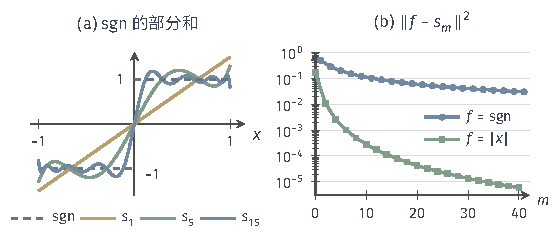
\includegraphics[width=94.9mm]{figures/02-abstract-mathematics/03-function-spaces/tikz/c1-legendre-truncation/figure.pdf}
  \caption{Legendre展开的截断。(a)$\operatorname{sgn}$（虚线）与部分和$s_1,s_5,s_{15}$，其中$s_1=\tfrac32x$；部分和是多项式，在跳跃点附近来回振荡。(b)截断误差$\lVert f-s_n\rVert_2^2$（对数纵轴）：$\operatorname{sgn}$取奇数$n$，$\lvert x\rvert$取偶数$n$。两条曲线都单调趋于零，有跳跃的$\operatorname{sgn}$下降慢得多。}
  \label{fig:ipspace-legendre-truncation}
\end{figure}

\paragraph{范数收敛不是点态收敛}
式~\eqref{eq:ipspace-tail-error}只控制$L^2$误差，不控制任何一点处的值。图~\ref{fig:ipspace-legendre-truncation}(a)中的部分和都是连续函数；若它们一致收敛，极限必然连续，而$\operatorname{sgn}$在$0$处跳跃，没有连续代表，所以部分和不一致收敛到$\operatorname{sgn}$，尽管$L^2$误差趋于零。在$x=0$处，每个部分和都是奇多项式，取值为$0$；而$\operatorname{sgn}$作为$L^2$元素在$0$处根本没有确定的值，谈不上收敛到什么。

更一般地，$L^2$中的元素是等价类，“展开在点$x_0$处收敛到$f(x_0)$”首先要求$f(x_0)$有意义，其次需要“点值受范数控制”这样的额外条件。由第~\ref{chap:normed-spaces}章，$L^2$收敛的序列有几乎处处收敛的子列，但整列部分和是否逐点收敛，要看具体的正交系与函数的正则性。点值读取何时连续，是第~\ref{chap:linear-functionals}章和第~\ref{chap:rkhs}章的问题；三角级数的逐点与一致收敛条件，在第~\ref{chap:fourier-transform}章讨论。

\section{本章小结}
\label{sec:ipspace-summary}

章首的两个问题都靠内积回答。内积的公理与维数无关，复情形约定对第二个变量线性、对第一个变量共轭线性；Cauchy--Schwarz不等式使$\sqrt{\langle f,f\rangle}$成为范数，并使内积连续。内积范数满足平行四边形恒等式，一致范数与$L^1$范数不满足，所以它们不来自任何内积。

Hilbert空间是在诱导范数下完备的内积空间，也就是范数来自内积的Banach空间。有限维时完备性自动成立，无限维时不然：有限支撑数列和平方积分下的连续函数都是不完备的内积空间。$L^2(\mu)$把平方可积函数的等价类收进来，乘积积分在Hölder不等式下有定义，诱导的正是$L^2$范数，由第~\ref{chap:normed-spaces}章的完备性直接成为Hilbert空间；计数测度下得到$\ell^2$。

在Hilbert空间的闭子空间上，最佳逼近存在且唯一：平行四边形恒等式使极小化序列成为柯西列，完备性给出极限，闭性保证极限留在子空间中。最近点由误差与子空间正交刻画，定义为正交投影，给出唯一的正交分解与勾股关系；有限支撑数列在$\ell^2$中的例子说明闭性不能去掉。一般闭凸集上最近点仍存在唯一，但正交条件要换成变分不等式，归卷五处理。

完备正交系只要求有限组合在范数下稠密，与只允许有限组合的代数基不同；它可以用“与所有方向正交的只有零”来检验，可分Hilbert空间的正交基至多可数，并可由Gram--Schmidt正交化得到。用内积系数展开时，有限截断就是正交投影，Bessel不等式控制系数；完备正交系给出依范数收敛的展开、Parseval等式和尾和形式的截断误差，并使空间与$\ell^2$同构；不完备时只恢复闭张成中的部分。范数收敛不等于点态收敛，Legendre部分和在$L^2$中收敛到$\operatorname{sgn}$，却不一致收敛。

这些结构为后面的章节准备了依据。第~\ref{chap:linear-functionals}章用正交投影证明连续线性泛函都能表示为内积，从而用内积表示观测；第~\ref{chap:fourier-transform}章和第~\ref{chap:wavelet-transform}章分别证明三角函数系与小波系的完备性；截断误差的衰减速度与函数光滑性的关系，由第~\ref{chap:function-approximation}章研究。

